% ============================================================
% 数电实验报告
% ============================================================

\documentclass[12pt]{ctexart}

% --- 宏包 ---
\usepackage{graphicx}
\usepackage{amsmath}
\usepackage{listings}
\usepackage{float}
\usepackage{booktabs}
\usepackage{siunitx}
\usepackage{fancyhdr}
\usepackage{caption}
\usepackage{subcaption}
\usepackage{hyperref}
\usepackage{makecell}
\usepackage{enumitem}

\sisetup{per-mode=symbol}

\graphicspath{{./figures/}}

\usepackage[left=2.5cm, right=2.5cm, top=2.5cm, bottom=2.5cm]{geometry}

\setlength{\jot}{6pt}
\linespread{1.5}
\setlist{nosep}

% --- 页眉页脚 ---
\pagestyle{fancy}
\fancyhead[C]{数字电子技术实验}
\fancyfoot[C]{\thepage}

\begin{document}

% ==================== 封面 ====================
\thispagestyle{empty}

\begin{figure}[t]
    \centering
    
\includegraphics[width=13cm]{logo1.png}
\end{figure}

\vspace*{\fill}
    \begin{center}
        \Huge\textbf{数字电子技术基础}

        \vspace{0.3cm}
        \Huge\textbf{实验报告}

        \vspace{1cm}
        \LARGE\textbf{实验一：TTL集成门电路逻辑变换}
    \end{center}
\vspace*{\fill}

\begin{table}[H]
    \centering
    \large
    \begin{tabular}{ll}
    \toprule
    \textbf{课程:} & 数字电子技术实验 \\
    \textbf{组员1:} & 郭浩然 2024303980 \\
    \textbf{组员2:} & 庞铭洋 2024302539 \\
    \textbf{组号:} & 15 \\
    \textbf{时间:} & \today \\
    \bottomrule
    \end{tabular}
\end{table}

\newpage

% ==================== 正文 ====================

\section{实验目的}

\begin{enumerate}
    \item 掌握使用门电路设计组合逻辑电路的基本方法，理解组合逻辑电路的分析与设计过程。
    \item 学习 Quartus II 软件的原理图输入设计流程，包括工程创建、元件放置、连线及编译等操作。
    \item 掌握利用波形仿真工具验证电路设计正确性的方法。
    \item 了解 DE0 开发板的基本使用方法，学习 FPGA 引脚锁定与程序下载流程。
\end{enumerate}

\section{实验要求}

使用门电路设计实现一位全加器，并在 FPGA 上实现该电路，通过拨动开关和观察 LED 灯验证其逻辑功能。

\section{实验设备}

\begin{itemize}
    \item Quartus II 开发软件
    \item DE0 开发板（FPGA 型号：Cyclone V 5CEBA4F23C7）
    \item USB 下载线及计算机
\end{itemize}

\section{实验原理}

\subsection{一位全加器}

一位全加器是实现两个一位二进制数及来自低位进位相加的组合逻辑电路。它有三个输入端：加数 $A$、加数 $B$ 和来自低位的进位输入 $C_0$；两个输出端：本位和 $S$ 以及向高位的进位输出 $C_1$。其真值表如表~\ref{tab:truth_table} 所示。

\begin{table}[H]
    \centering
    \caption{一位全加器真值表}
    \label{tab:truth_table}
    \begin{tabular}{ccc|cc}
        \toprule
        $A$ & $B$ & $C_0$ & $S$ & $C_1$ \\
        \midrule
        0 & 0 & 0 & 0 & 0 \\
        0 & 0 & 1 & 1 & 0 \\
        0 & 1 & 0 & 1 & 0 \\
        0 & 1 & 1 & 0 & 1 \\
        1 & 0 & 0 & 1 & 0 \\
        1 & 0 & 1 & 0 & 1 \\
        1 & 1 & 0 & 0 & 1 \\
        1 & 1 & 1 & 1 & 1 \\
        \bottomrule
    \end{tabular}
\end{table}

\subsection{逻辑表达式}

根据真值表，利用卡诺图化简可得一位全加器的逻辑表达式：

\begin{align}
    S &= A \oplus B \oplus C_0 \label{eq:S} \\
    C_1 &= AB + (A \oplus B) C_0 \label{eq:C1}
\end{align}

其中，式~\eqref{eq:S} 表示本位和为三个输入的异或；式~\eqref{eq:C1} 表示进位输出在至少有两个输入为 1 时为高电平。

\subsection{门电路实现}

根据上述逻辑表达式，一位全加器可使用以下门电路实现：

\begin{itemize}
    \item 2 个二输入异或门（XOR2）：分别计算 $A \oplus B$ 和 $(A \oplus B) \oplus C_0$
    \item 2 个二输入与门（AND2）：分别计算 $AB$ 和 $(A \oplus B) C_0$
    \item 1 个二输入或门（OR2）：计算 $AB + (A \oplus B) C_0$
\end{itemize}

完整的电路原理图如图~\ref{fig:circuit} 所示。

\begin{figure}[H]
    \centering
    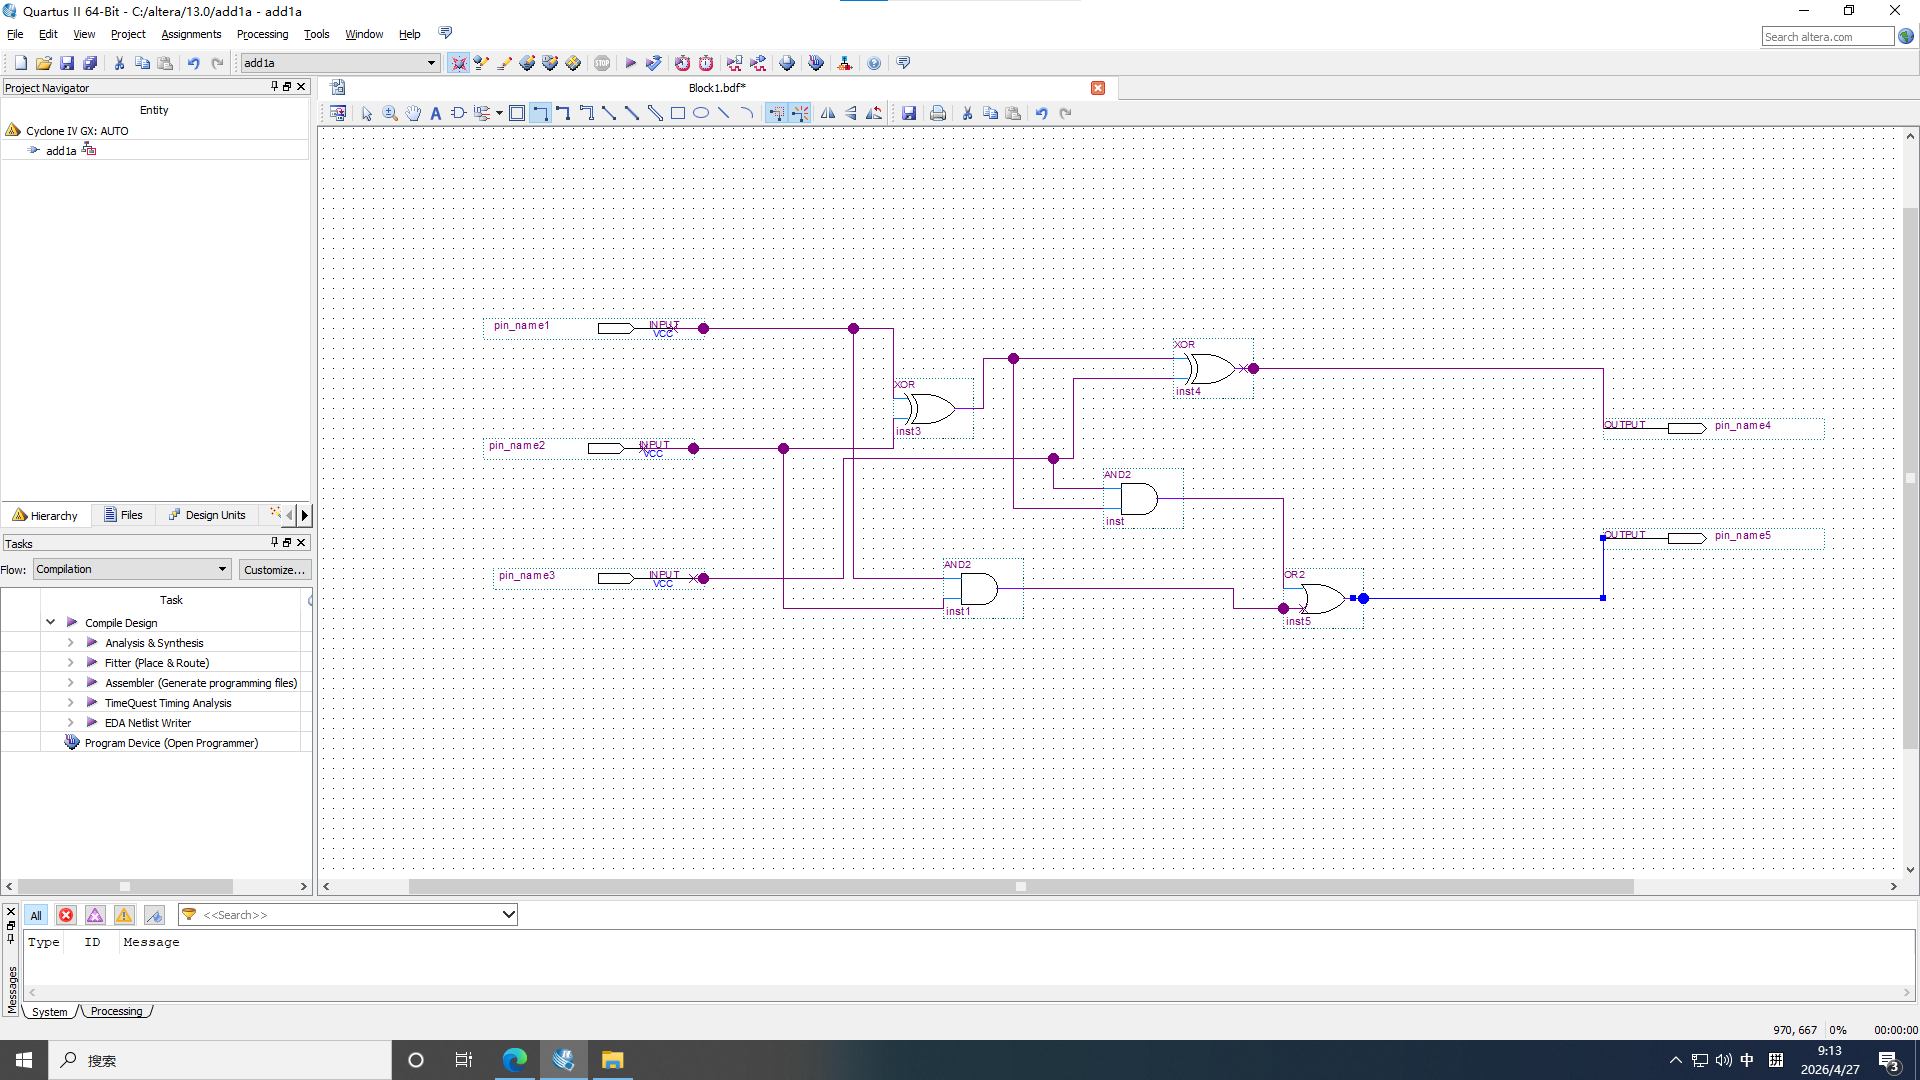
\includegraphics[width=0.85\textwidth]{circuit_diagram.png}
    \caption{一位全加器电路原理图}
    \label{fig:circuit}
\end{figure}

\section{实验内容}

\subsection{创建工程与绘制原理图}

\subsubsection{创建 Quartus II 工程}

启动 Quartus II 软件，通过 \textbf{File $\rightarrow$ New Project Wizard} 创建新工程。在项目信息设置对话框中，设置工程存放路径、项目名称（如 \texttt{add1a}），并确保顶层实体名称与项目名称一致。在目标器件设置中选择 Cyclone V 系列的 \texttt{5CEBA4F23C7} 器件，以匹配 DE0 开发板上的 FPGA 芯片。

\subsubsection{绘制原理图}

工程创建完成后，通过 \textbf{File $\rightarrow$ New $\rightarrow$ Block Diagram/Schematic File} 新建原理图文件。在原理图编辑窗口中，通过元件库（Libraries）放置以下元件：

\begin{itemize}
    \item \texttt{primitives/logic/xor2}：2 个二输入异或门
    \item \texttt{primitives/logic/and2}：2 个二输入与门
    \item \texttt{primitives/logic/or2}：1 个二输入或门
    \item \texttt{primitives/pin/input}：3 个输入引脚（命名为 A、B、C0）
    \item \texttt{primitives/pin/output}：2 个输出引脚（命名为 S、C1）
\end{itemize}

按照图~\ref{fig:circuit} 所示的电路结构连接各元件，完成后保存原理图文件。绘制好的原理图如图~\ref{fig:schematic} 所示。

\begin{figure}[H]
    \centering
    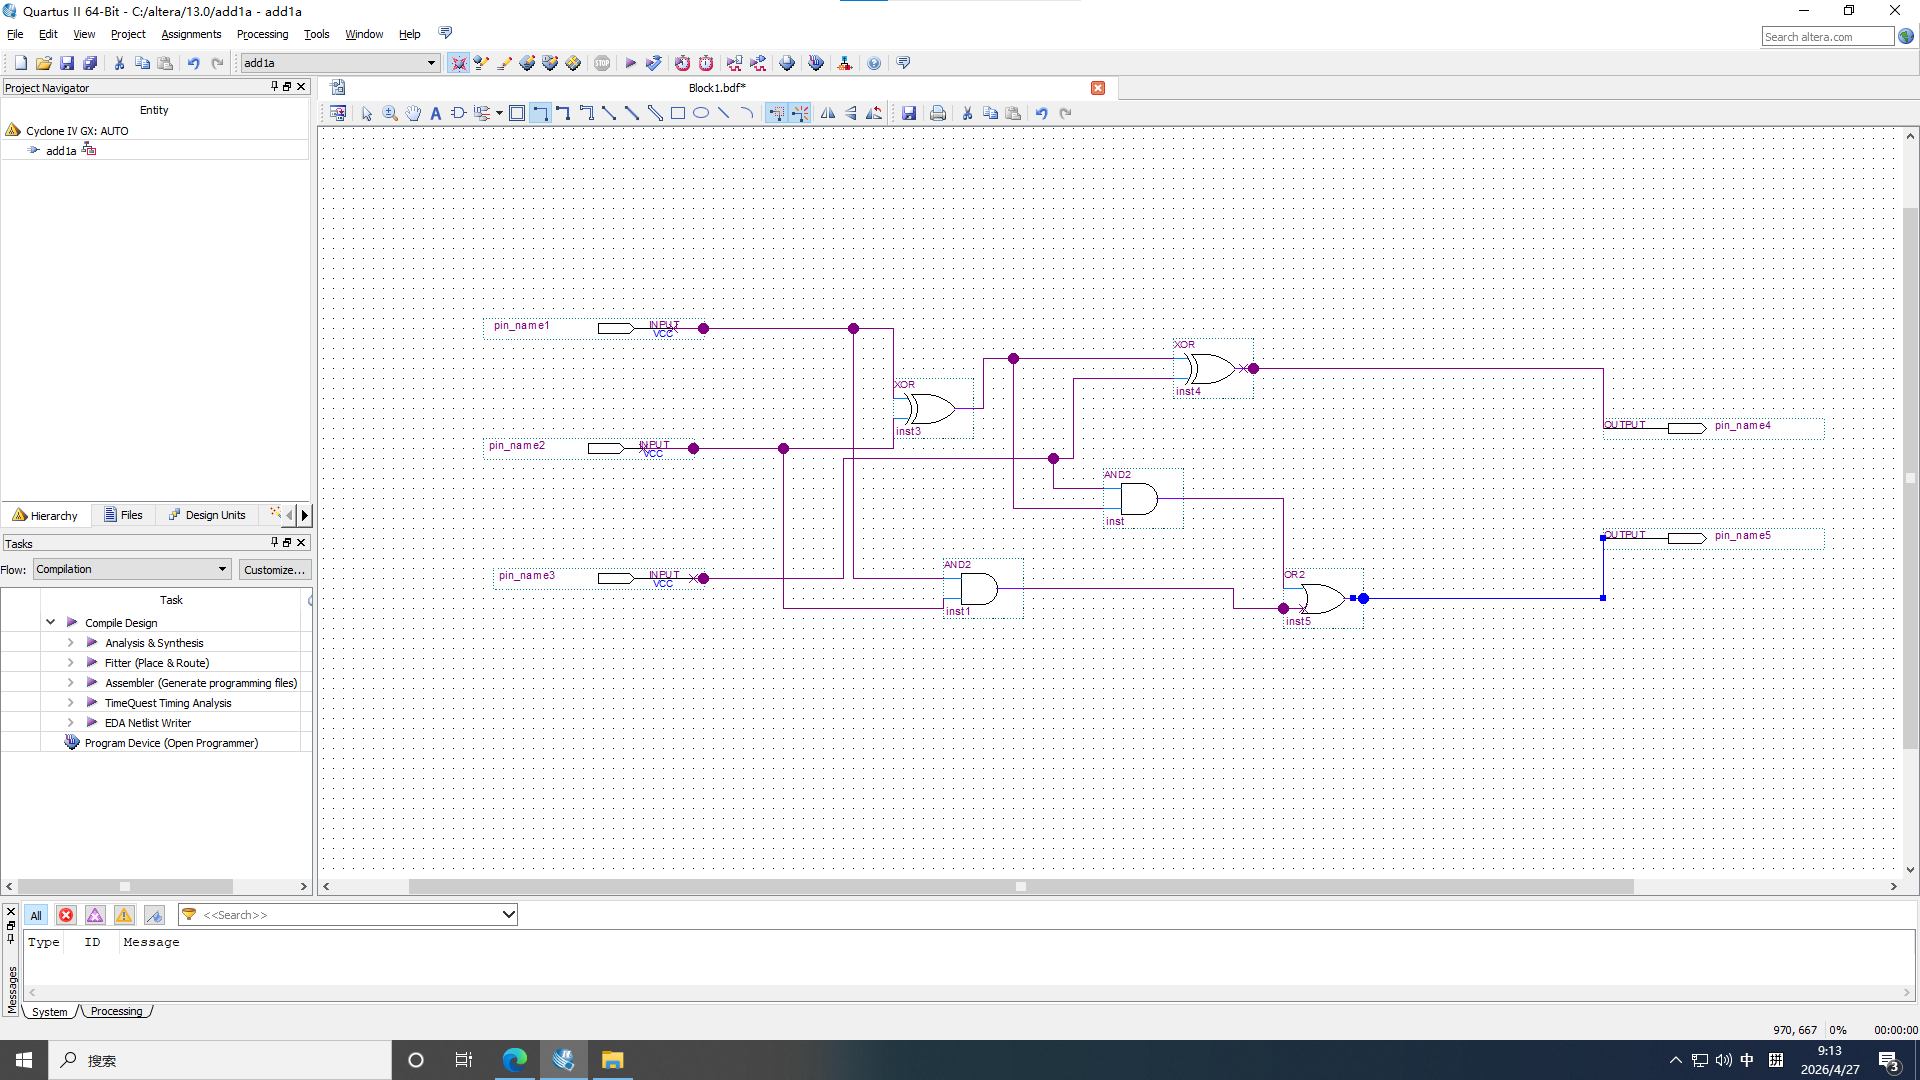
\includegraphics[width=0.85\textwidth]{circuit_diagram.png}
    \caption{Quartus II 中绘制的一位全加器原理图}
    \label{fig:schematic}
\end{figure}

\subsection{编译与波形仿真}

\subsubsection{编译}

原理图绘制完成后，点击工具栏中的编译图标或执行 \textbf{Process $\rightarrow$ Start Compilation} 进行全编译。编译过程包括综合（Synthesis）、适配（Fitter）和汇编（Assembler）等步骤。编译成功后，Quartus II 界面会显示编译报告，确认无错误（Error）即可进行下一步操作。

\subsubsection{波形仿真}

通过 \textbf{File $\rightarrow$ New $\rightarrow$ Verification/Debugging $\rightarrow$ Vector Waveform File} 新建波形仿真文件（.vwf）。使用 \textbf{Edit $\rightarrow$ Insert $\rightarrow$ Insert Node or Bus} 添加仿真信号，在 Node Finder 中选择 \texttt{Pins:all} 获取所有输入输出节点。

设置仿真激励信号的计数值：A 信号每 10ns 翻转一次，B 信号每 20ns 翻转一次，C0 信号每 40ns 翻转一次。这样可以遍历真值表中的所有 8 种输入组合。

执行 \textbf{Processing $\rightarrow$ Start Simulation} 运行仿真，观察输出波形。仿真结果如图~\ref{fig:simulation} 所示。

\begin{figure}[H]
    \centering
    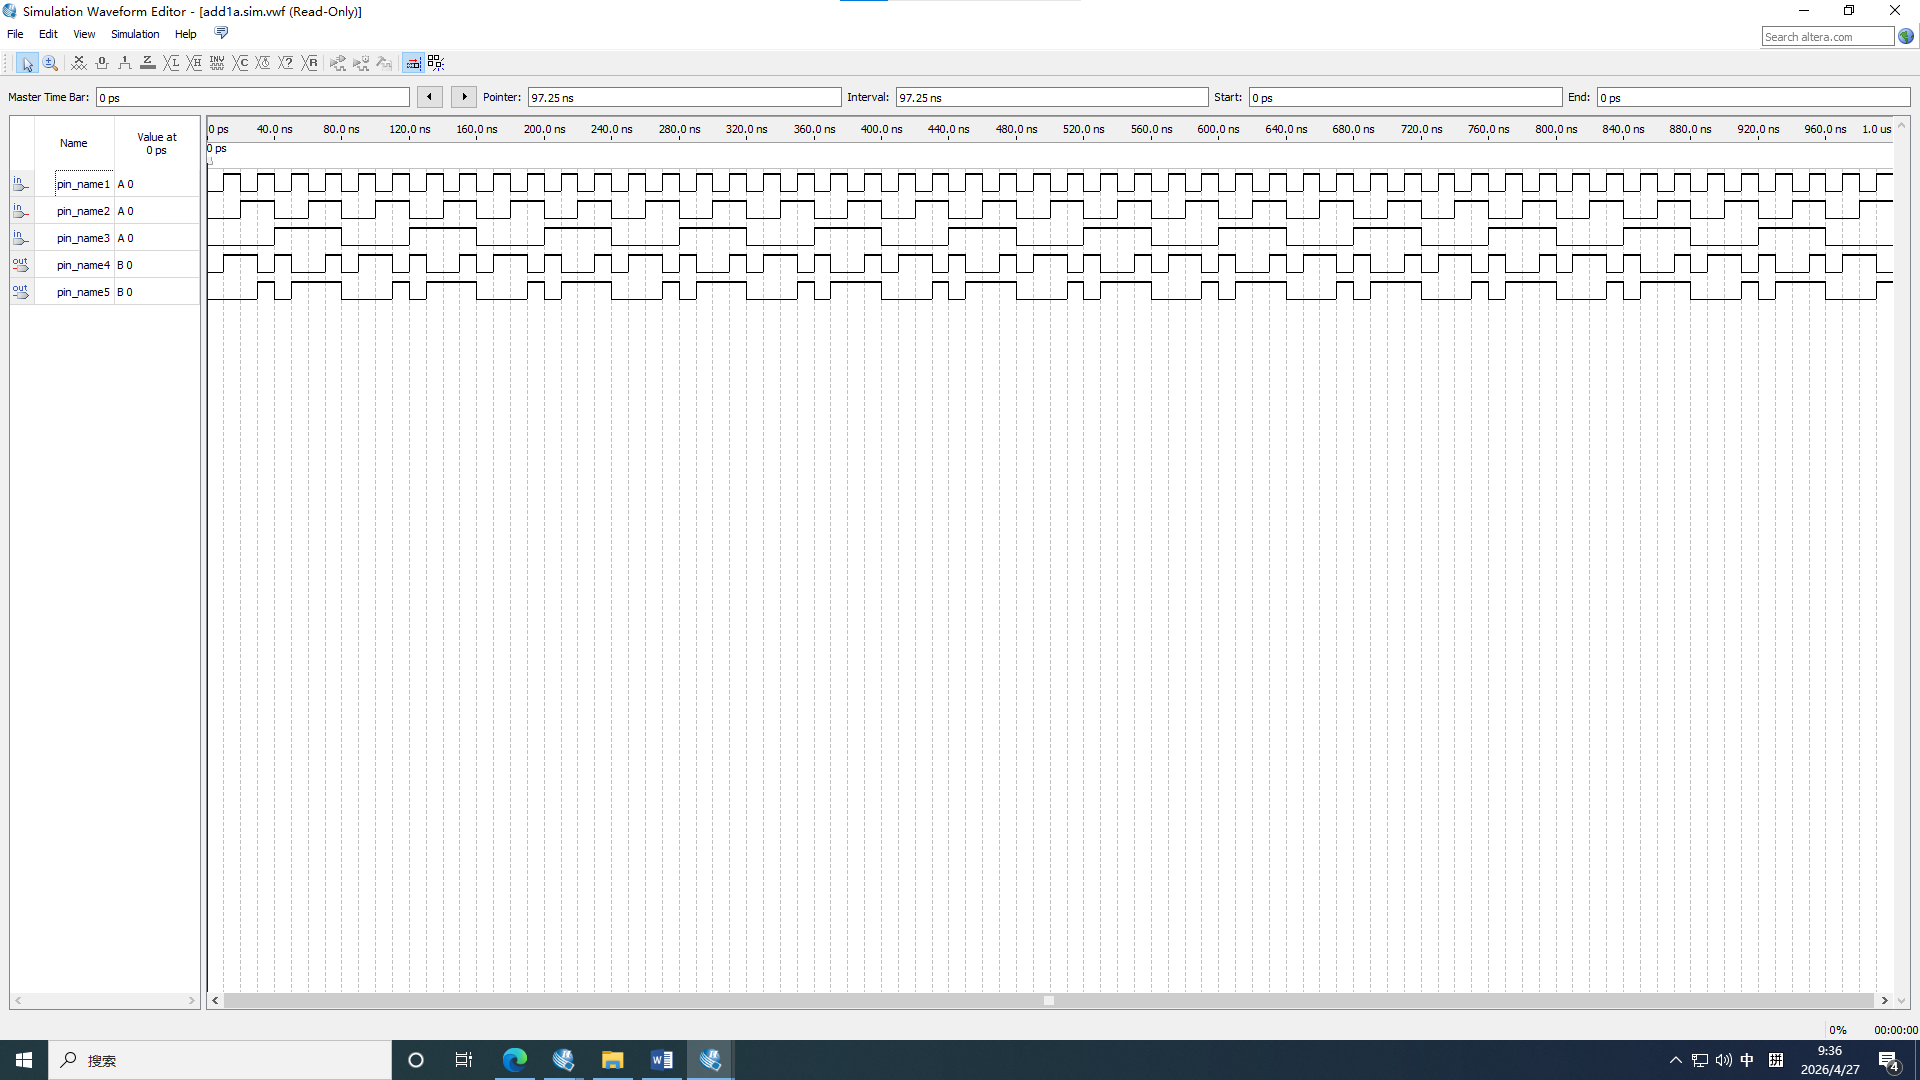
\includegraphics[width=\textwidth]{simulation.png}
    \caption{一位全加器波形仿真结果}
    \label{fig:simulation}
\end{figure}

从仿真波形可以看出，在 0--80ns 的仿真时间内，输入 A、B、C0 的 8 种组合对应的输出 S 和 C1 均与真值表一致，验证了电路设计的正确性。

\subsection{引脚锁定与 FPGA 下载验证}

\subsubsection{引脚锁定}

根据 DE0 开发板的引脚分配表，使用 \textbf{Assignments $\rightarrow$ Pin Planner} 将设计中的端口与 FPGA 物理引脚对应绑定。引脚分配如表~\ref{tab:pin_assign} 所示。

\begin{table}[H]
    \centering
    \caption{引脚分配表}
    \label{tab:pin_assign}
    \begin{tabular}{cccc}
        \toprule
        \textbf{端口名} & \textbf{功能} & \textbf{FPGA 引脚} & \textbf{对应硬件} \\
        \midrule
        A & 输入 & PIN\_U13 & SW0 \\
        B & 输入 & PIN\_V13 & SW1 \\
        C0 & 输入 & PIN\_T13 & SW2 \\
        S & 输出 & PIN\_J1 & LEDG[0] \\
        C1 & 输出 & PIN\_J2 & LEDG[1] \\
        \bottomrule
    \end{tabular}
\end{table}

引脚锁定后，需重新执行全编译以生成包含引脚信息的编程文件（.sof）。

\subsubsection{FPGA 下载}

将计算机通过 USB 线连接至 DE0 开发板的 J8 接口，按下红色电源开关 SW10 启动开发板。在 Quartus II 中执行 \textbf{Tools $\rightarrow$ Programmer}，在编程器对话框中选择 JTAG 模式，点击 \textbf{Hardware Setup} 选择 \texttt{USB-Blaster [USB-0]} 下载接口。加载编译生成的 .sof 文件，勾选 \texttt{Program/Configure}，点击 \textbf{Start} 开始下载。下载成功后的 Programmer 界面如图~\ref{fig:fpga} 所示。

\begin{figure}[H]
    \centering
    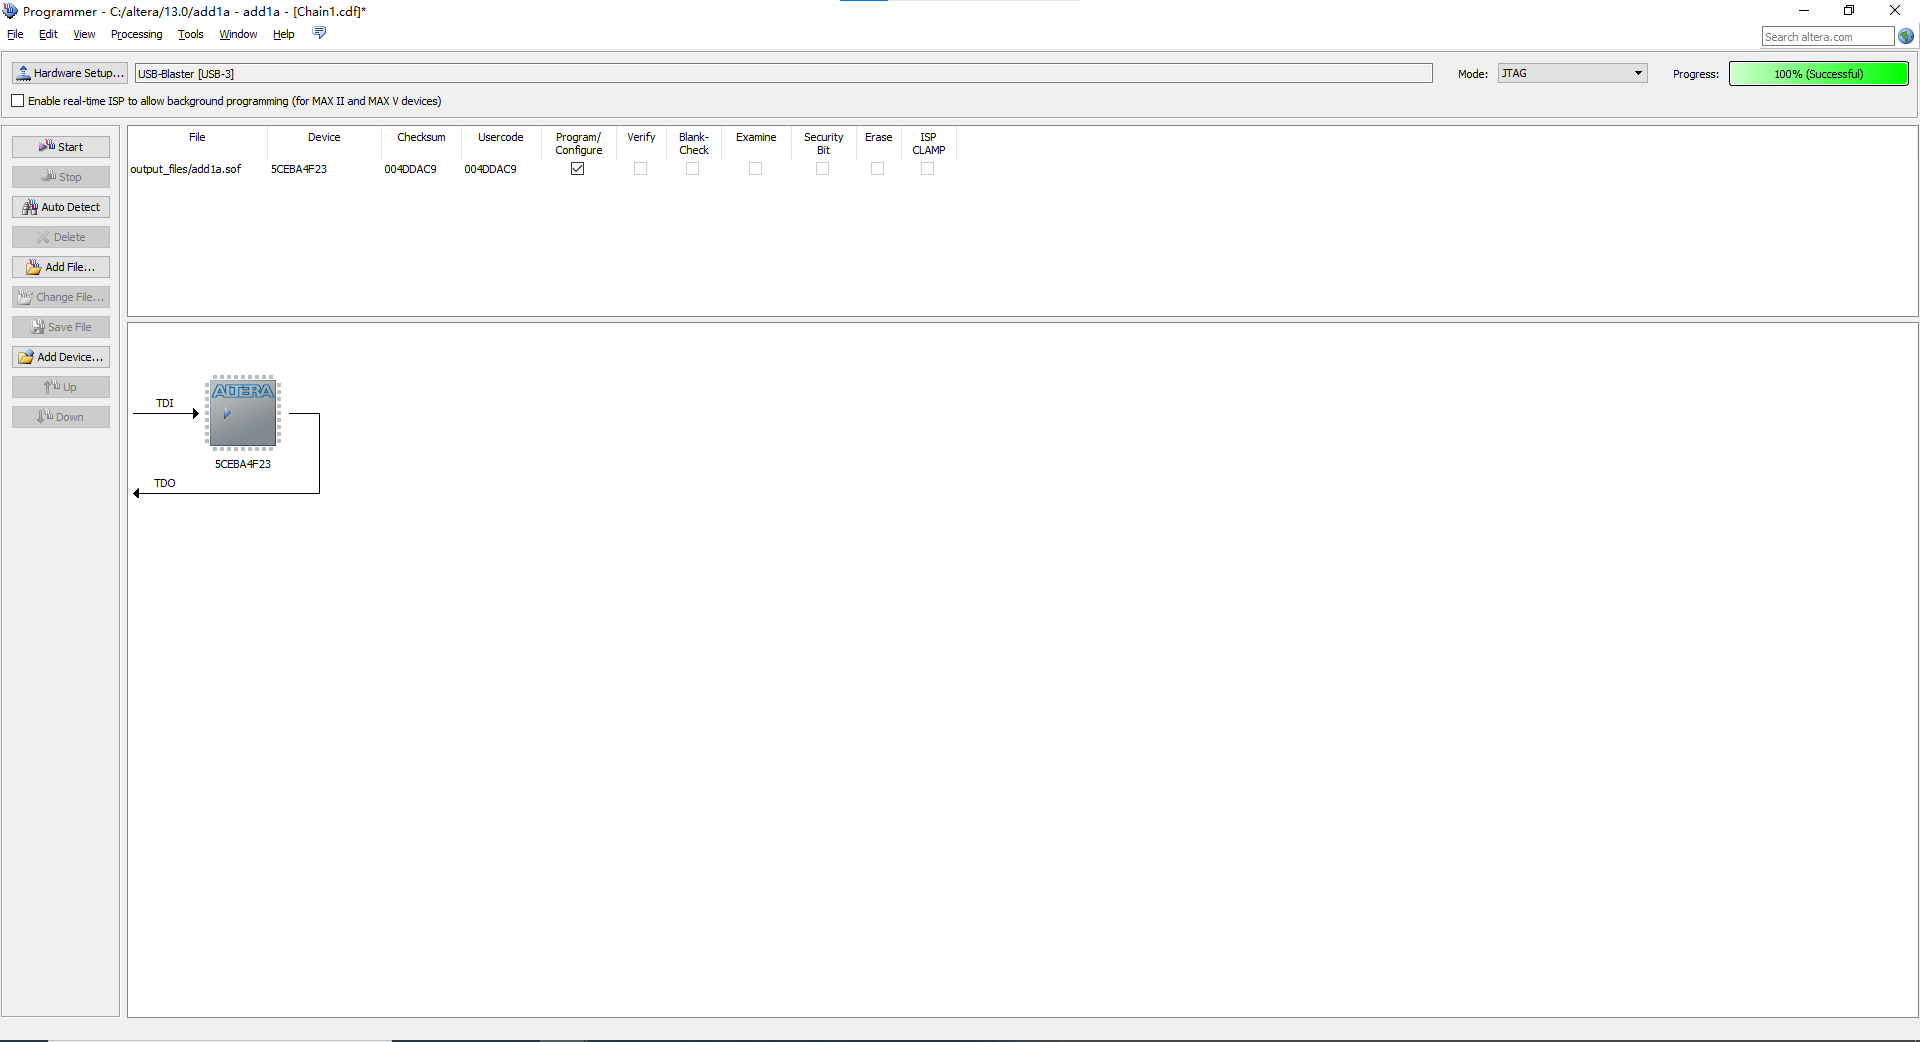
\includegraphics[width=0.7\textwidth]{FPGA.png}
    \caption{FPGA 下载成功界面}
    \label{fig:fpga}
\end{figure}

\subsubsection{硬件验证}

下载完成后，在 DE0 开发板上通过拨动开关 SW0、SW1、SW2 分别控制输入 A、B、C0 的电平，观察 LEDG[0]（S）和 LEDG[1]（C1）的亮灭状态。选取四种典型输入组合进行验证，结果如图~\ref{fig:out00}--\ref{fig:out11} 所示。

\begin{figure}[H]
    \centering
    \begin{subfigure}[b]{0.48\textwidth}
        \centering
        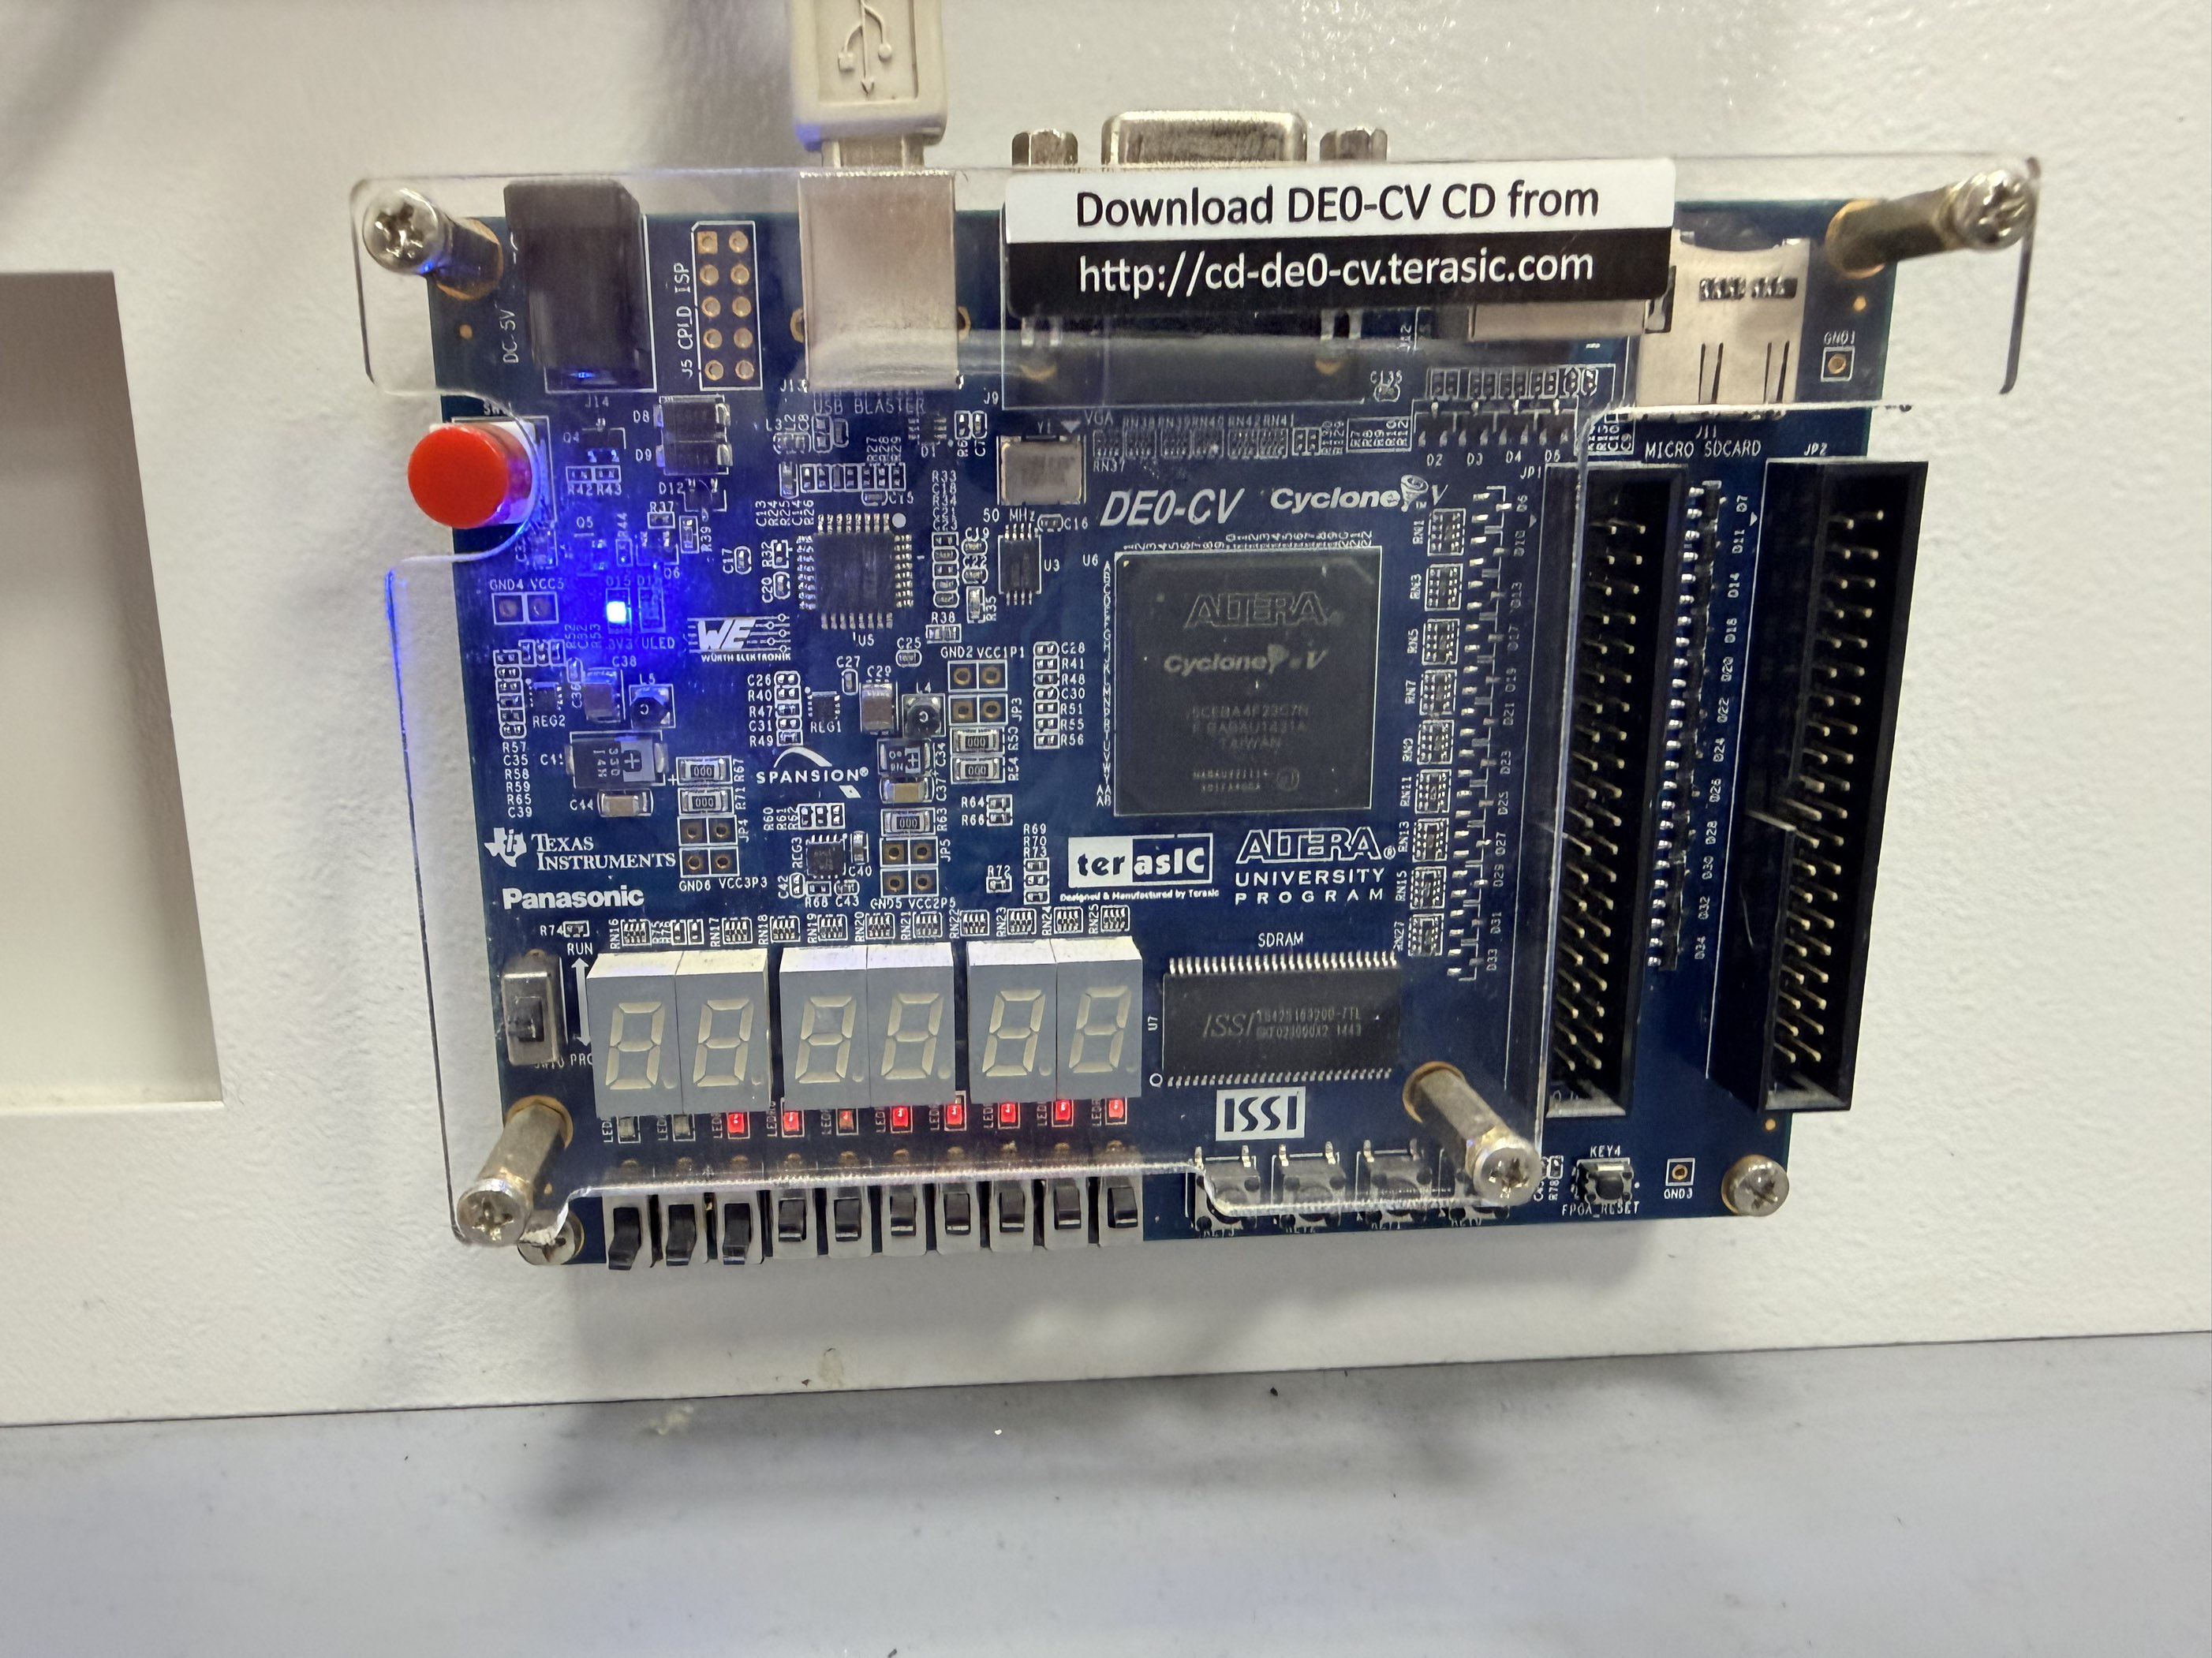
\includegraphics[width=\textwidth]{out00.png}
        \caption{$A=0, B=0, C_0=0 \Rightarrow S=0, C_1=0$}
        \label{fig:out00}
    \end{subfigure}
    \hfill
    \begin{subfigure}[b]{0.48\textwidth}
        \centering
        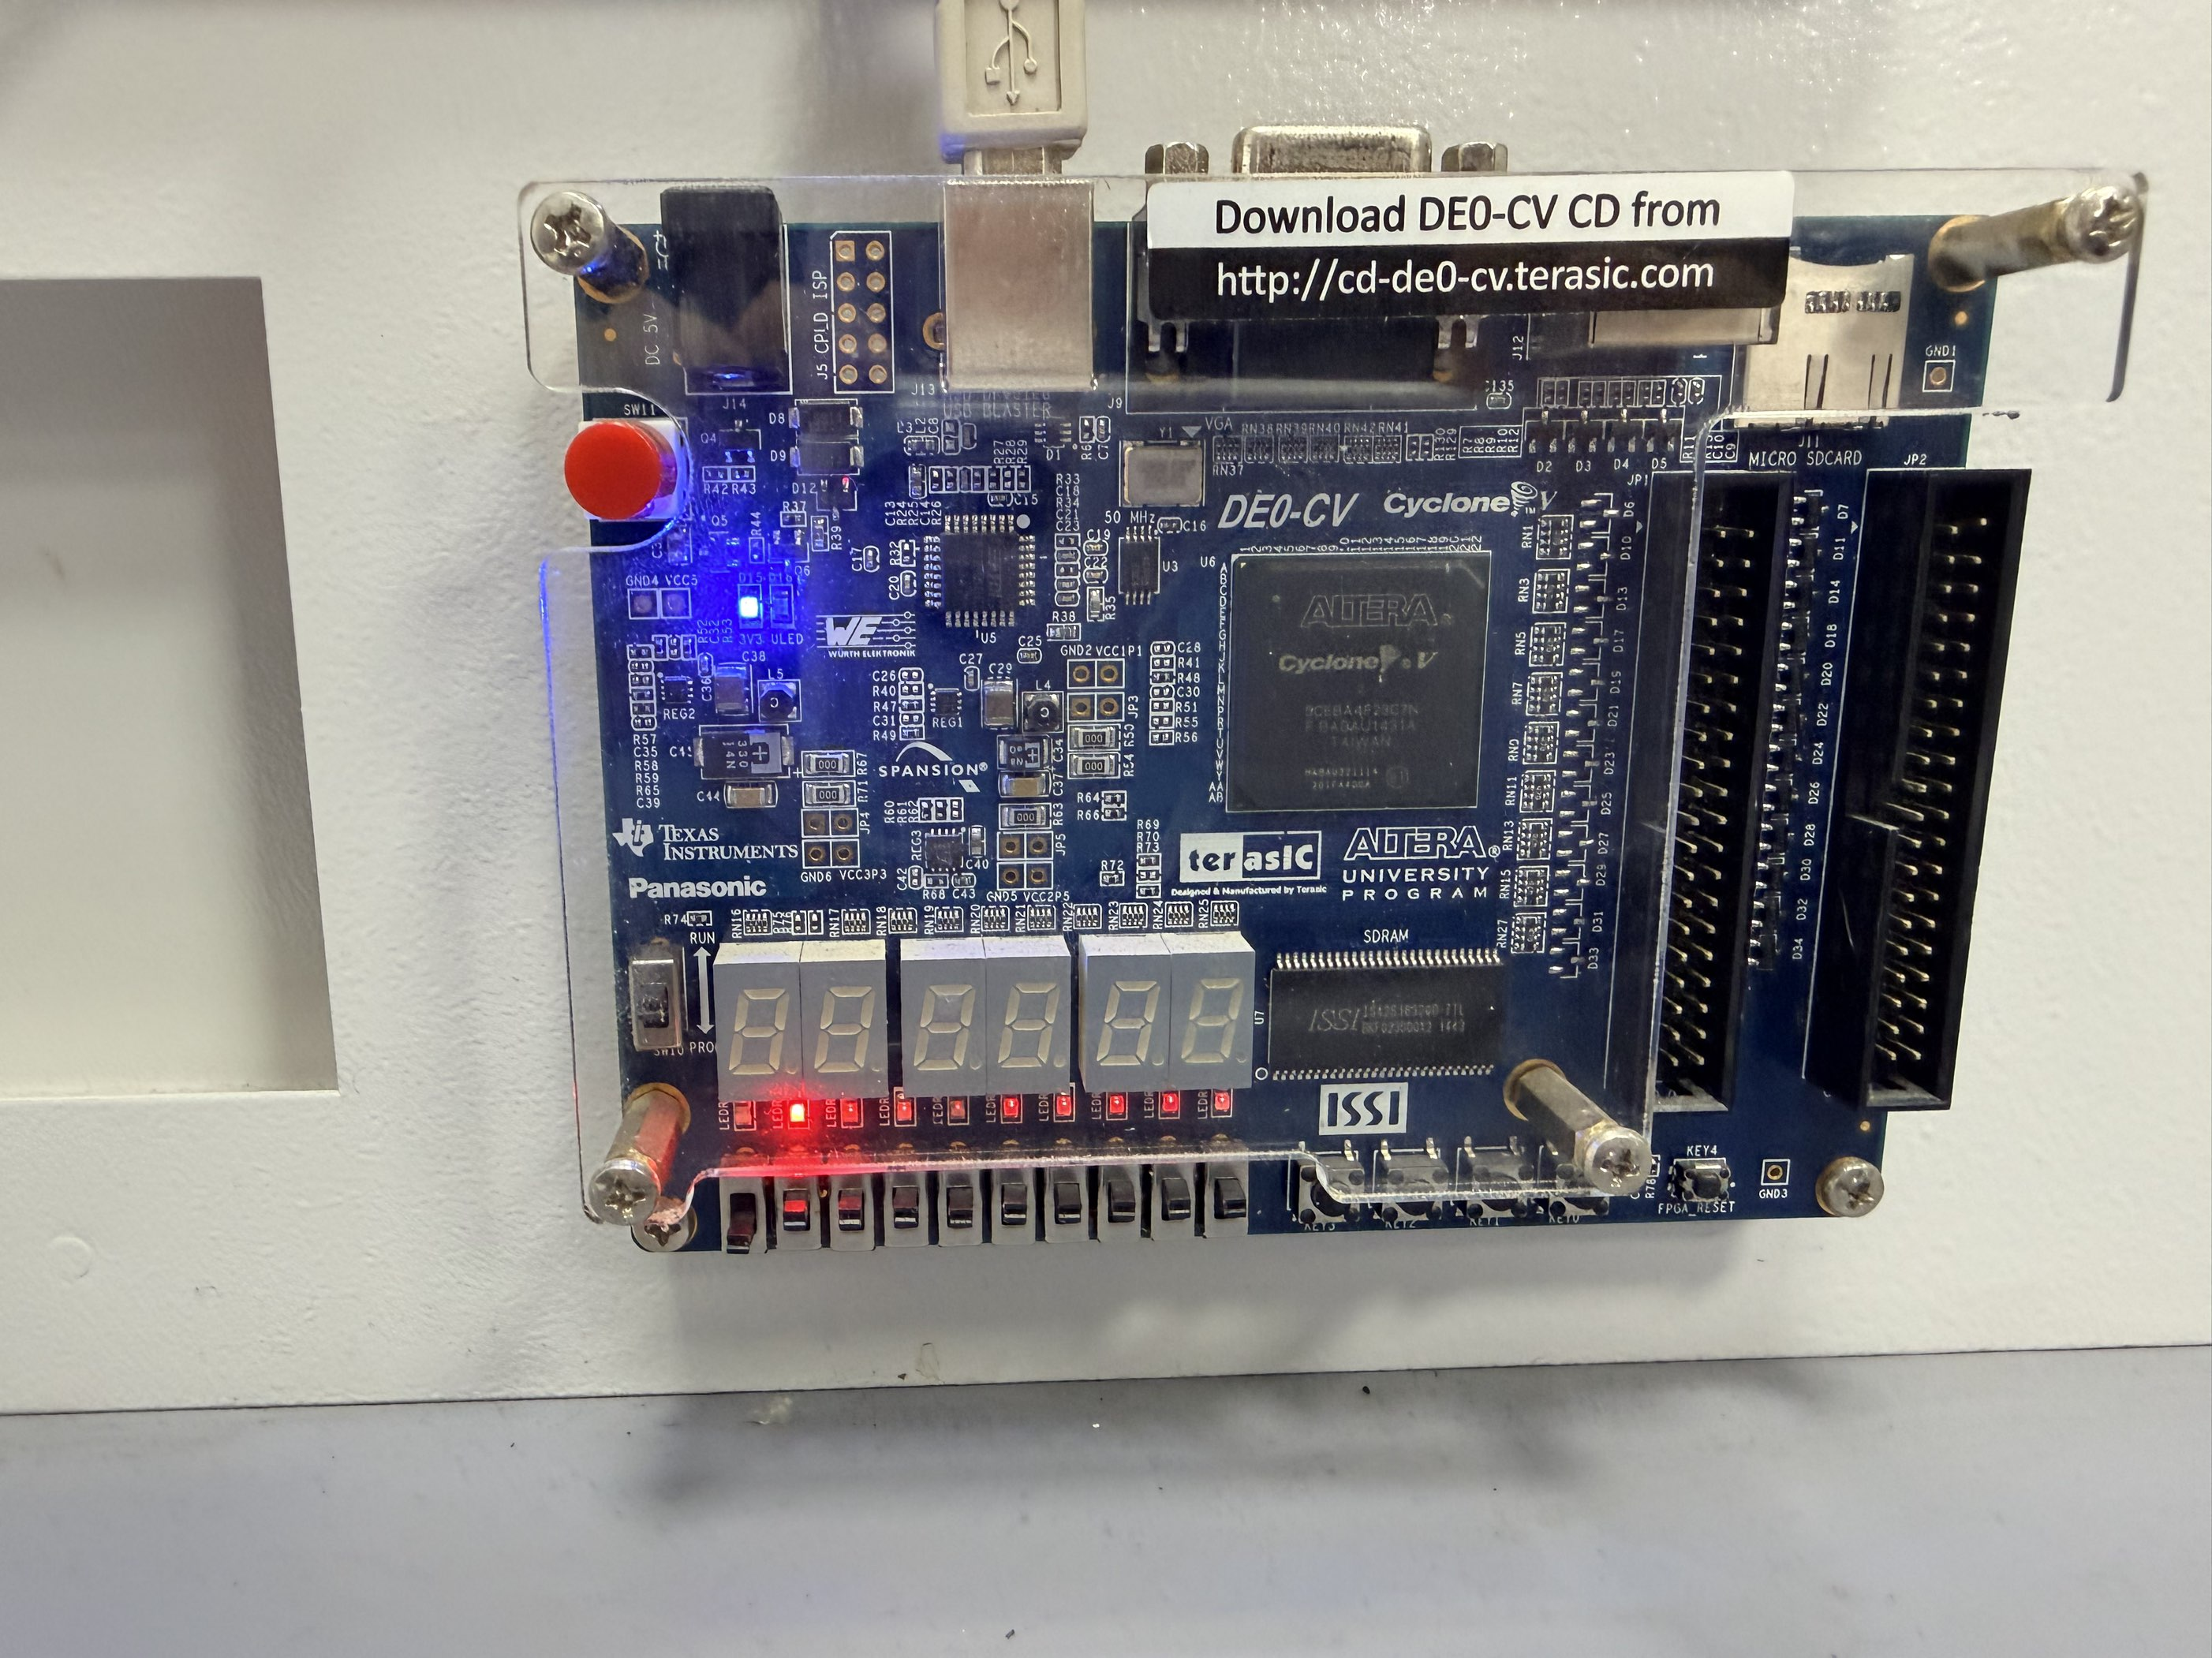
\includegraphics[width=\textwidth]{out01.png}
        \caption{$A=0, B=0, C_0=1 \Rightarrow S=1, C_1=0$}
        \label{fig:out01}
    \end{subfigure}

    \vspace{0.5cm}

    \begin{subfigure}[b]{0.48\textwidth}
        \centering
        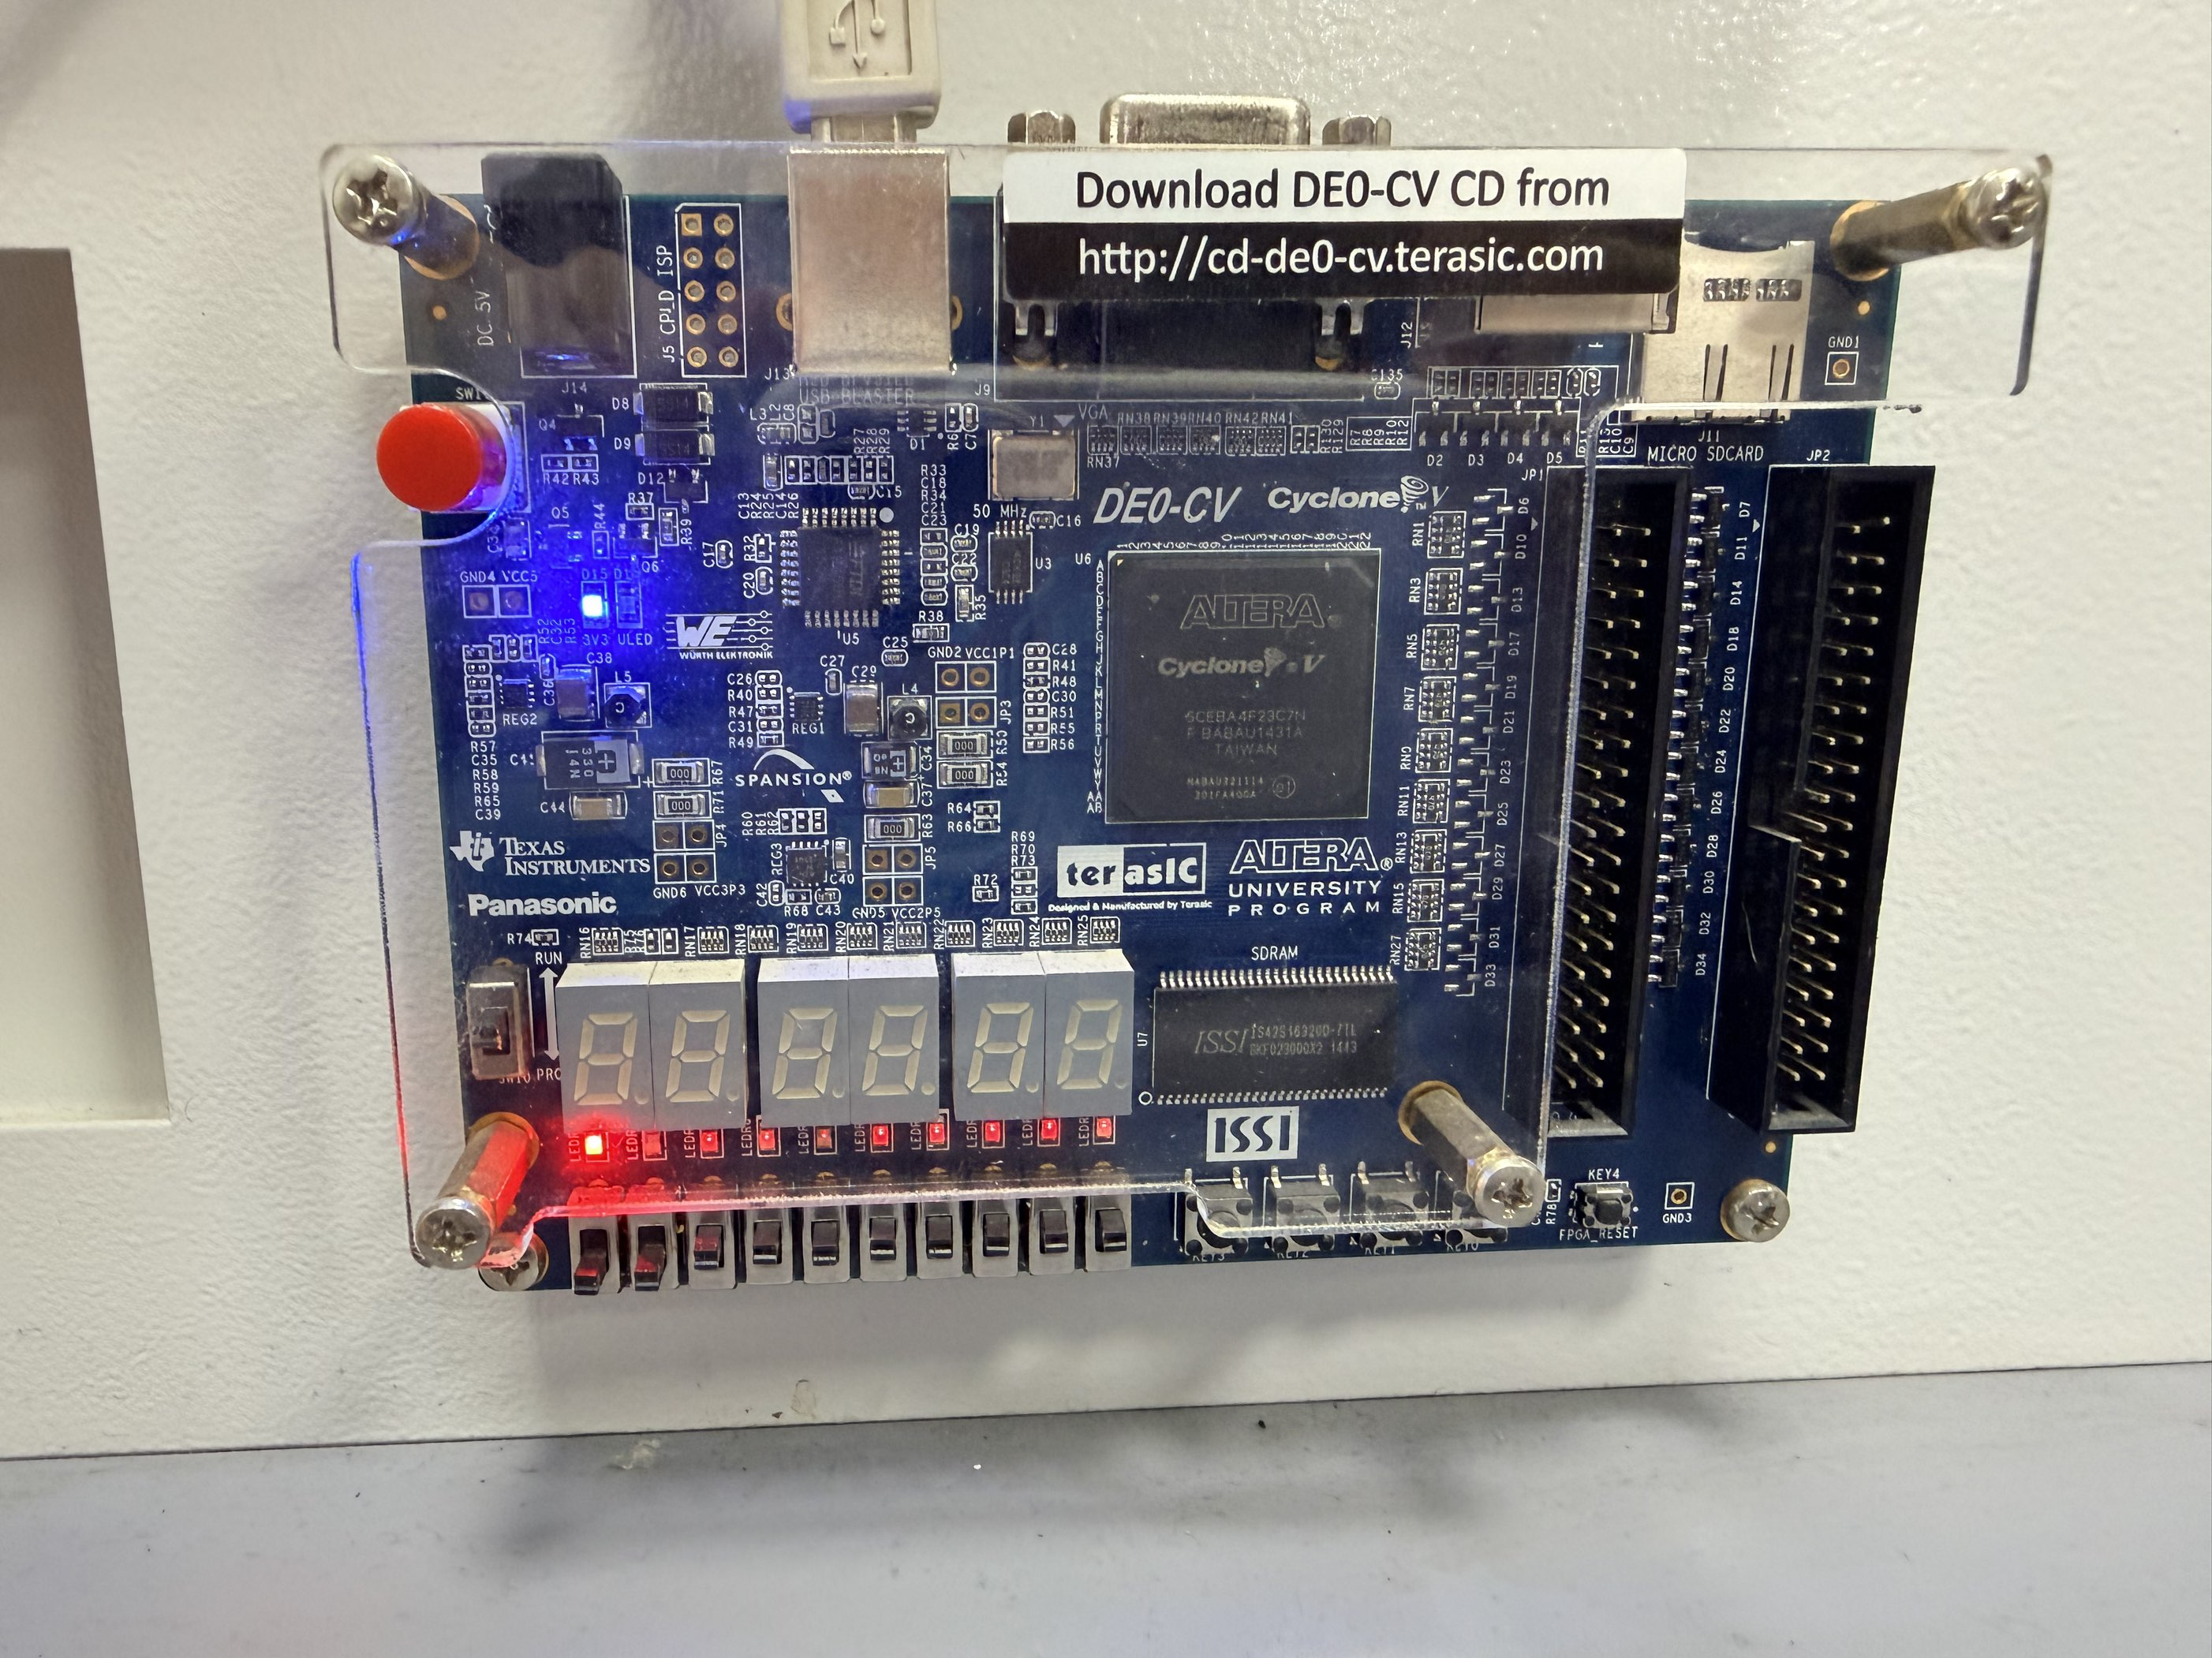
\includegraphics[width=\textwidth]{out10.png}
        \caption{$A=1, B=0, C_0=0 \Rightarrow S=1, C_1=0$}
        \label{fig:out10}
    \end{subfigure}
    \hfill
    \begin{subfigure}[b]{0.48\textwidth}
        \centering
        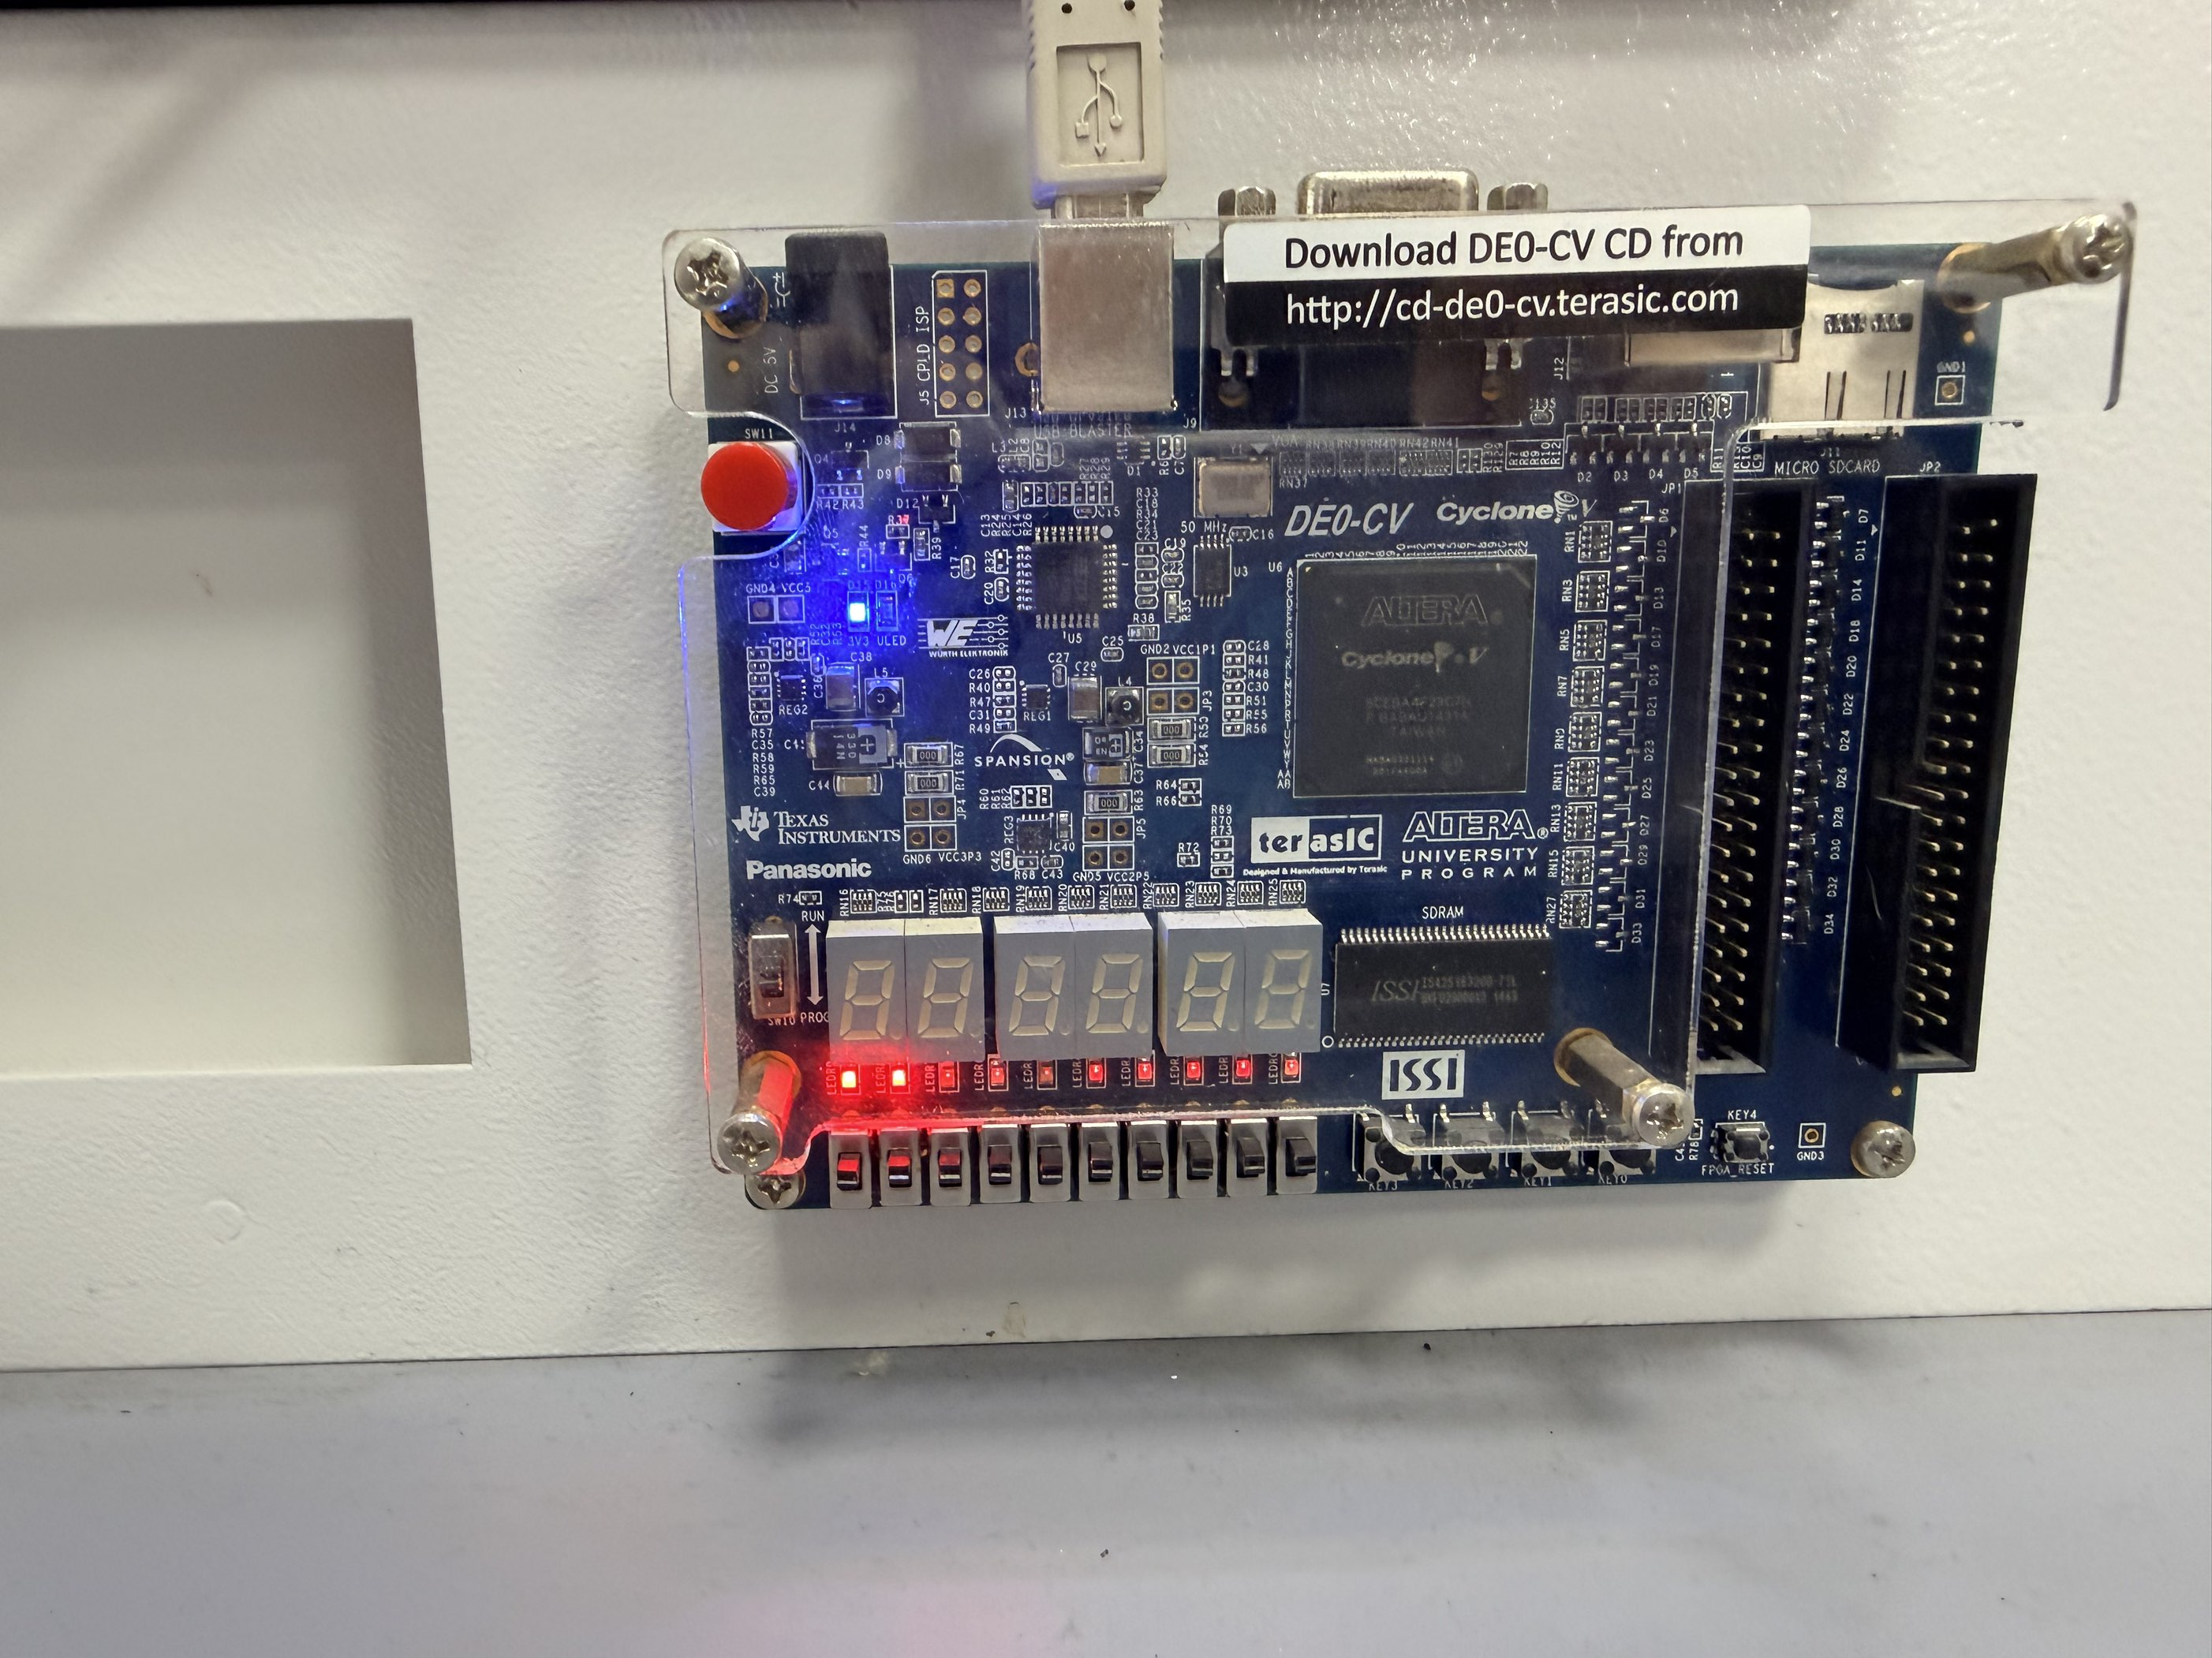
\includegraphics[width=\textwidth]{out11.png}
        \caption{$A=1, B=1, C_0=1 \Rightarrow S=1, C_1=1$}
        \label{fig:out11}
    \end{subfigure}
    \caption{FPGA 硬件验证结果}
    \label{fig:fpga_results}
\end{figure}

从硬件验证结果可以看出，四种输入组合下 LED 灯的亮灭状态均与真值表一致，证明所设计的一位全加器在 FPGA 上正确实现了逻辑功能。

\section{实验过程中的问题}

\begin{enumerate}
    \item \textbf{波形仿真失败}：在首次进行波形仿真时，仿真器报错提示 \texttt{"Can't continue timing simulation because the design has not been successfully compiled for the simulator"}，如图~\ref{fig:sim_fail} 所示。经排查发现，是因为在创建工程时未正确选择目标器件，导致编译产物与仿真器不兼容。重新创建工程并正确选择 Cyclone V 5CEBA4F23C7 器件后，仿真顺利完成。

    \begin{figure}[H]
        \centering
        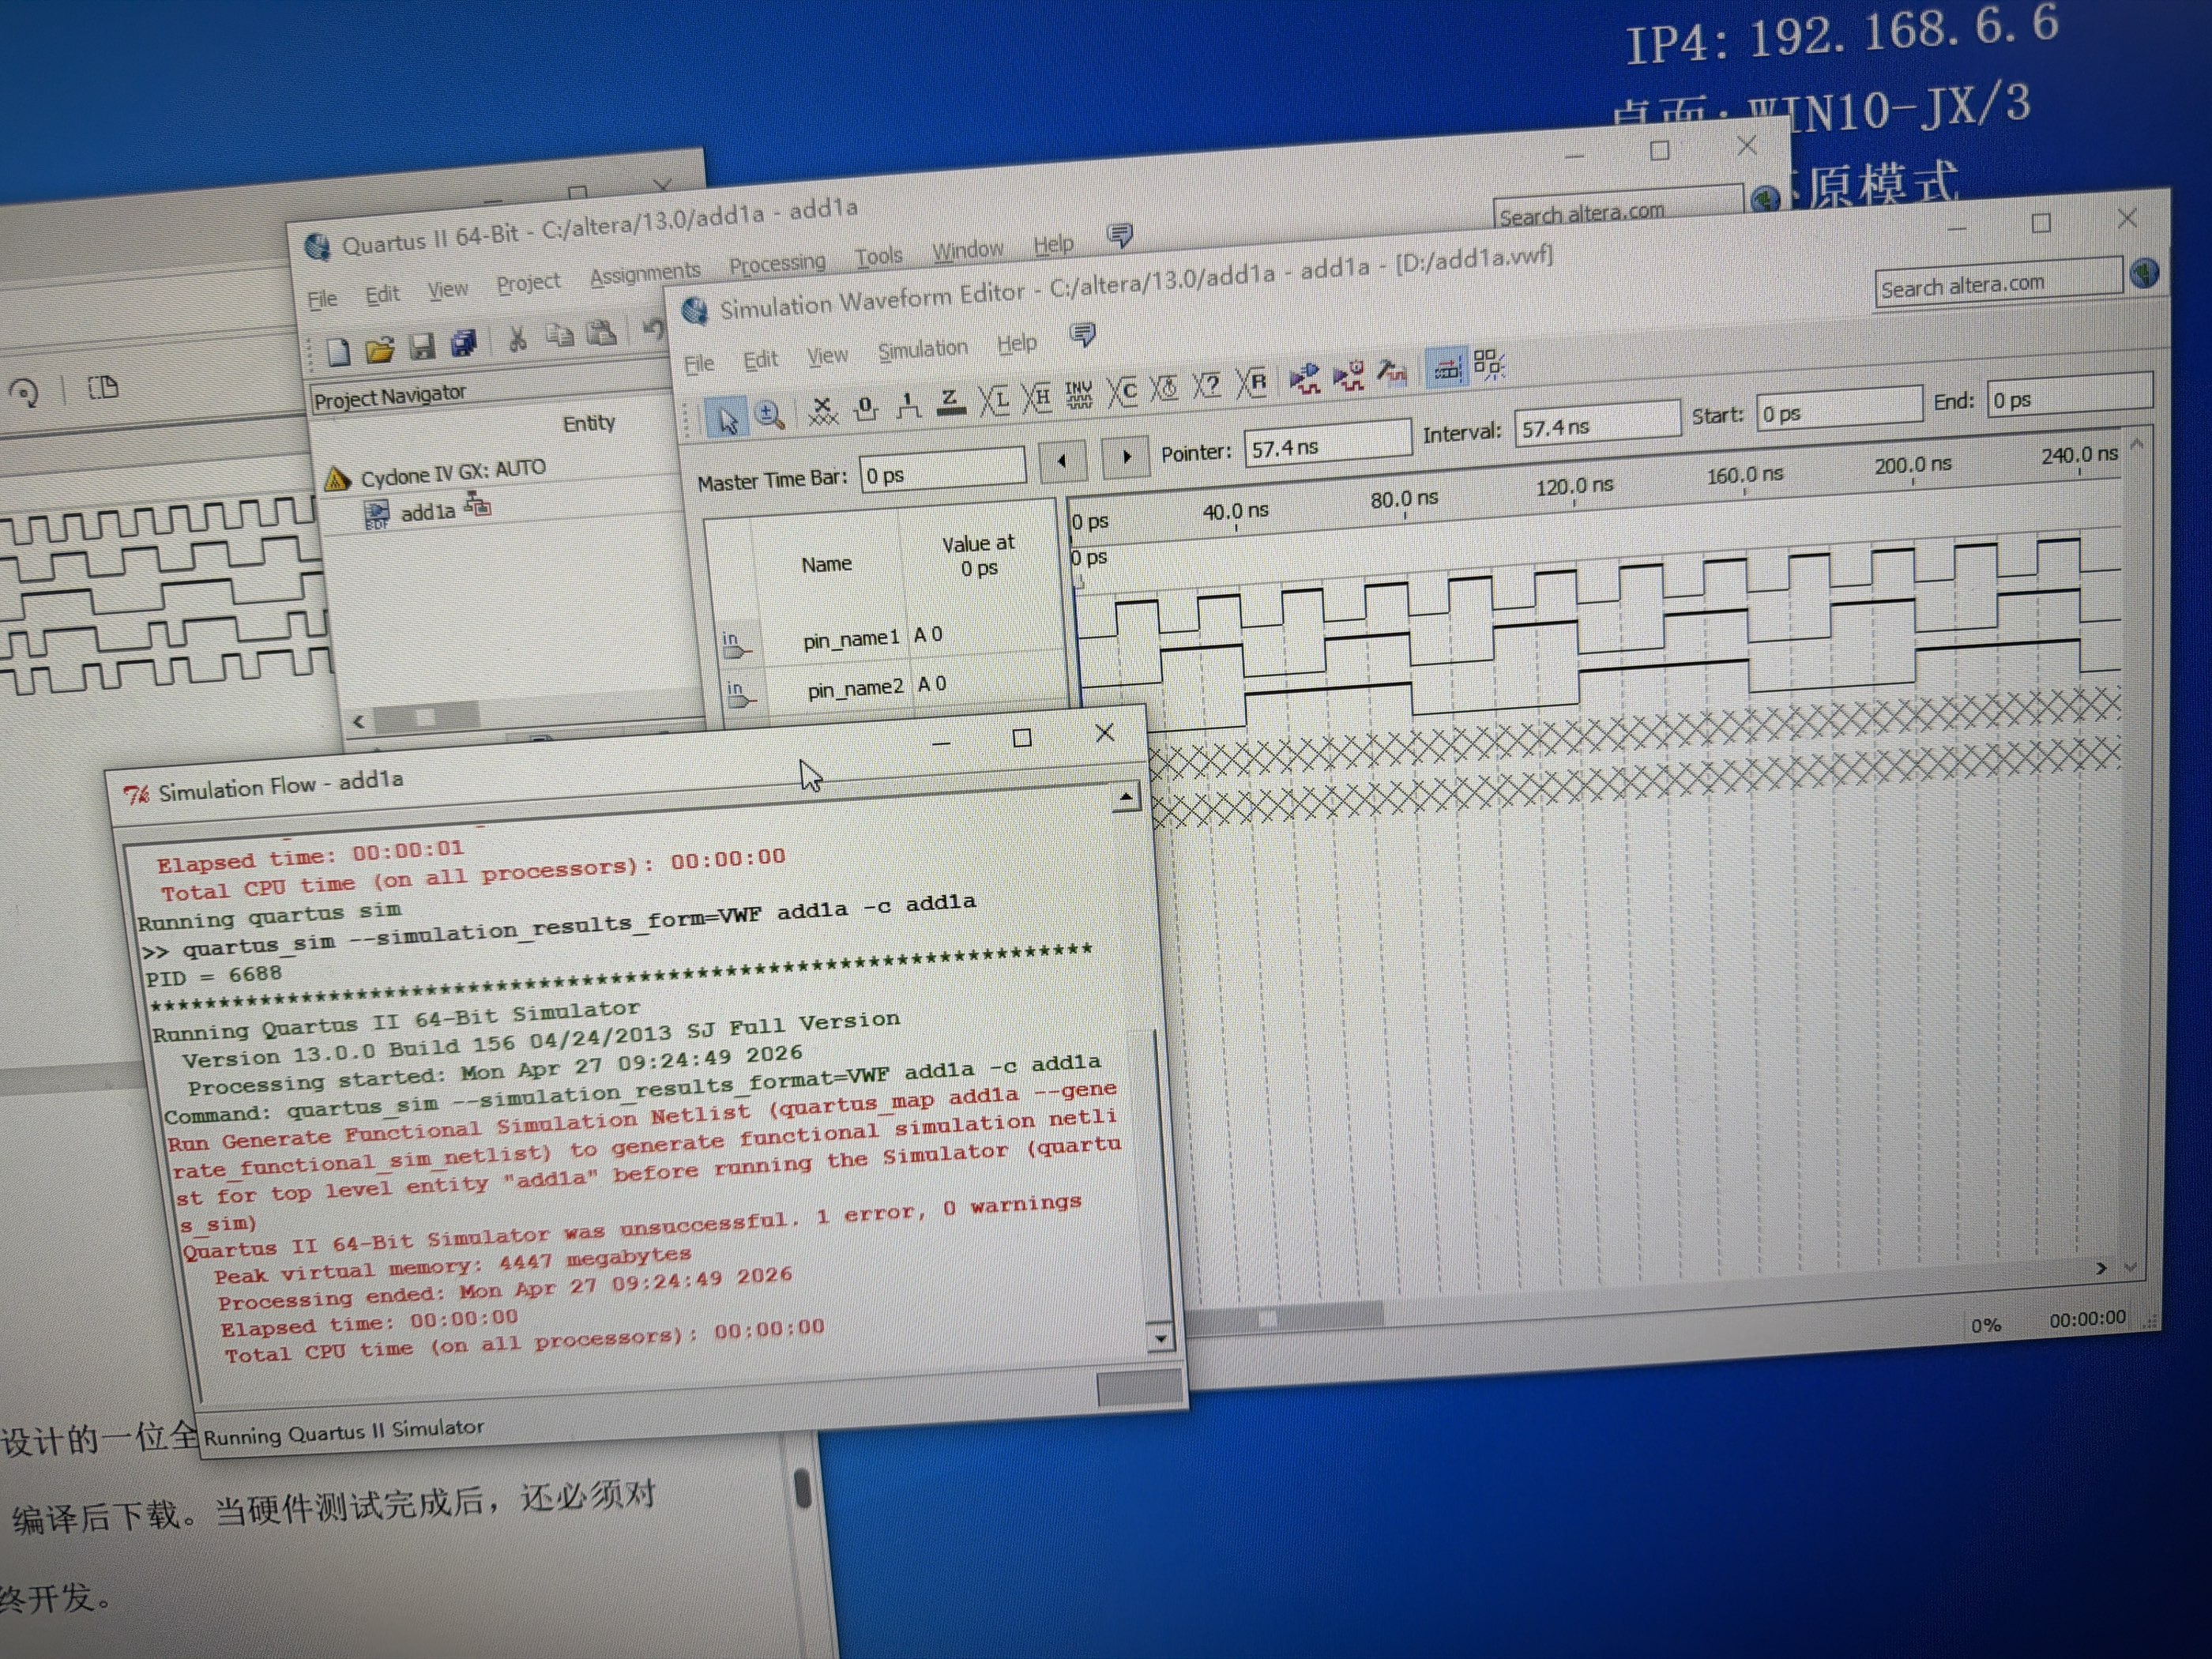
\includegraphics[width=0.7\textwidth]{simulation_fail.png}
        \caption{仿真失败截图（器件选择错误）}
        \label{fig:sim_fail}
    \end{figure}

    \item \textbf{引脚锁定后未重新编译}：在完成引脚锁定后直接进行下载，发现 FPGA 上的 LED 灯输出与预期不符。原因是引脚锁定后需要重新执行全编译，才能将新的引脚信息写入编程文件。重新编译后问题解决。
\end{enumerate}

\section{心得体会}

\begin{enumerate}
    \item 通过本次实验，掌握了使用门电路设计组合逻辑电路的基本方法。从真值表推导逻辑表达式，再到选择合适的门电路实现，整个过程加深了对组合逻辑电路设计的理解。
    \item 学习了 Quartus II 软件的完整设计流程，包括原理图输入、编译、波形仿真、引脚锁定和 FPGA 下载等环节。这些技能为后续更复杂数字电路的设计奠定了基础。
    \item 在实验过程中遇到的仿真失败问题，提醒我在创建工程时必须仔细核对目标器件型号，这是后续所有操作的前提。同时，引脚锁定后需要重新编译这一细节也加深了我对 FPGA 设计流程的理解。
    \item 通过将理论设计与实际硬件验证相结合，直观地感受到了数字电路从设计到实现的完整过程，增强了理论联系实际的能力。
\end{enumerate}

\end{document}
